\documentclass{article}
\usepackage[T1]{fontenc}
\usepackage{lmodern}
\usepackage{graphicx}
\usepackage{amsmath,amssymb}
\usepackage[a4paper,margin=2cm]{geometry}
\usepackage[absolute,overlay]{textpos}
\setlength{\TPHorizModule}{1mm}
\setlength{\TPVertModule}{1mm}
\usepackage[indonesian]{babel}
\usepackage{hyperref}
\setlength{\emergencystretch}{2em}
% unit: Halaman 26

\begin{document}

% === Halaman 26 (llm) ===

\vspace{210.87mm}

Carrier File \vspace{10mm} Carrier File with Hidden Message

% deskripsi: Ilustrasi konsep steganografi yang menunjukkan proses penyisipan pesan rahasia dari sebuah file teks ('myhiddenmessage.txt') ke dalam sebuah 'Carrier File' untuk menghasilkan 'Carrier File with Hidden Message'.
% bbox normalisasi: [0.1600, 0.1200, 0.8300, 0.8300]
\begin{textblock*}{140.70mm}(33.60mm,35.64mm)
\noindent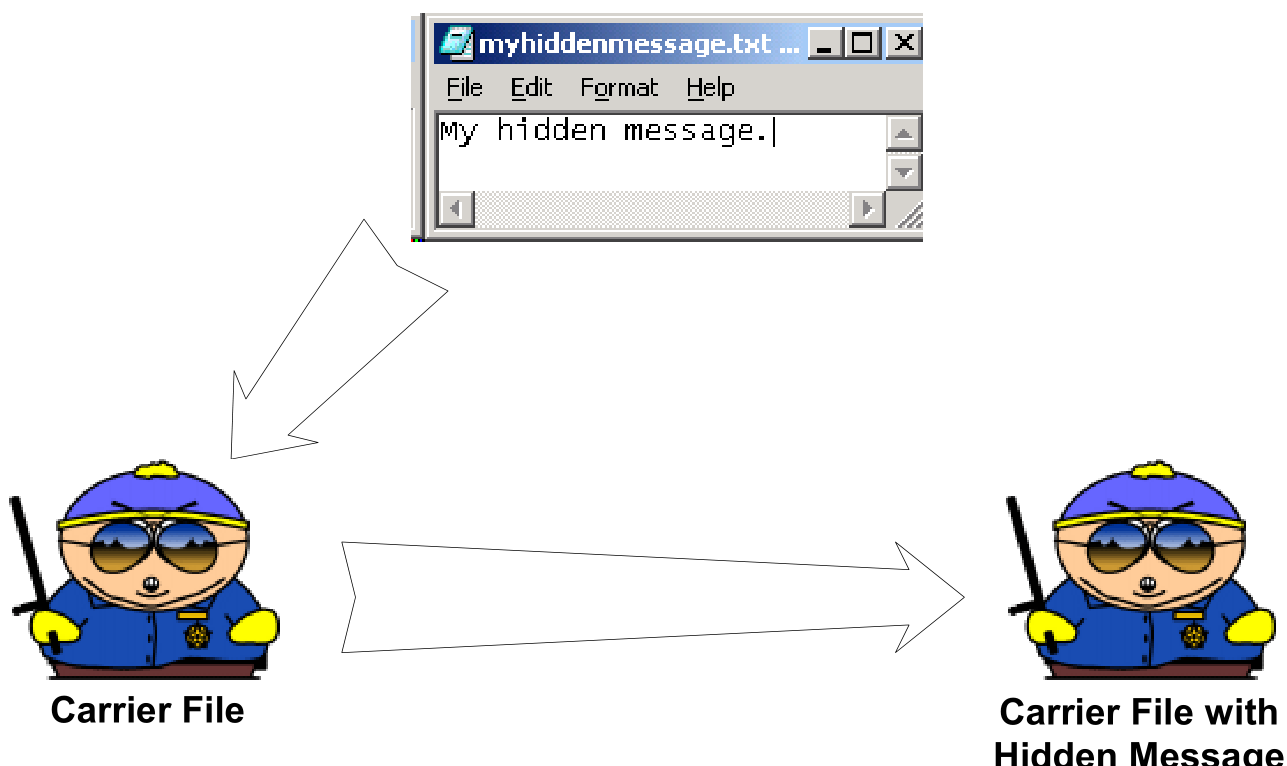
\includegraphics[width=140.70mm,height=210.87mm]{../../images/llm/page_026_img_01.png}%
\end{textblock*}

\end{document}
